%  This LaTeX template is based on T.J. Hitchman's work which is itself based on Dana Ernst's template.  
% 
% --------------------------------------------------------------
% Skip this stuff, and head down to where it says "Start here"
% --------------------------------------------------------------
 
\documentclass[12pt]{article}
\usepackage[margin=1in]{geometry} 
\usepackage{amsmath,amsthm,amssymb}
\usepackage{graphicx}
\usepackage{listings}
\usepackage{hyperref}
\usepackage[nottoc]{tocbibind}

\hypersetup{
	colorlinks=true,
	linkcolor=blue,
	filecolor=magenta,      
	urlcolor=cyan,
}
\newenvironment{statement}[2][Statement]{\begin{trivlist}
\item[\hskip \labelsep {\bfseries #1}\hskip \labelsep {\bfseries #2.}]}{\end{trivlist}}
\begin{document} 
\title{Midterm Progress Report}
\author{Eric L. Lee, Yu-Cheng Weng, Can Jiang, Shu-Hao Chang} 
\maketitle

\section{Abstract}
Our proposal proposes that we want to perform link prediction on network structured data.

In this period, we have collected data and established our evaluation framework. We implemented 6 baselines model in the 8 different data sets. Besides, we perform data analysis and visualize our data set.

In the following three weeks, we will focus on implmenting factorization model and state-of-the-art methods. And try to further improve our result. 

\section{How to Reproduce Our Result}
We believe reproducibility is very important when it comes to research. So, we carefully record all of our experiment results in github.

All of our result we presented in the following sections can be easily reproduced using this github repo. \\

\url{https://github.com/miamiasheep/Purdue\_ML\_Course\_Project}
\\
If you want to reproduce all of our result (including data analysis part), you can type the following command: 
\begin{lstlisting}
python script.py
\end{lstlisting}
If you want to reproduce the result of certain data sets, you can type the following command:
\begin{lstlisting}
python main.py --input [file1,file2,...] --goal [auc/f1]
\end{lstlisting}
If you want to draw the graph of a network, you can type the following command:
\begin{lstlisting}
python main.py --input [file] --draw [N(Integer)]
\end{lstlisting}
When N is larger, the sample network will be larger.

\section{Data Analysis}

\subsection {Data Set}
We collect 8 different data sets and all the data sets are very unique and have different characteristics. And table \ref{tab:info} shows basic statistics of each data set.
\subsubsection{Facebook}
This is a data set downloaded from SNAP(Staford NEtwork Analysis Project)\cite{snapnets}. The data is an egonet in facebook. Each node represent an account in facebook and each link represents friendship in facebook.
\subsubsection{Power}
Power is  an electrical grid of western US\cite{small_world}.
\subsubsection{NS}
NS is a collaboration network of resarchers who publish paper on network sciences \cite{Newman_2006}.
\subsubsection{PB}
PB is a network of US political blogs.\cite{pb}
\subsubsection{Router}
Router is a router-level Internet.\cite{router}
\subsubsection{USAir}
USAir is a network of US air lines. \cite{usair}
\subsubsection{Yeast}
Yeast is a protein-protein interaction network in yeast.\cite{yeast}

\subsubsection{Celegan}
Celegan is a neural network of C. elegans.\cite{small_world}

\begin{table}
\begin{center}
	\begin{tabular}{|c|c|c|c|c|}
		\hline
		data set & nodes & edges & average degree & max degree \\
		Facebook & 4039 & 88234 & 21.85 & 1045 \\
		Power & 4941 & 6595 & 1.33 & 19 \\
		NS & 1461 & 2742 & 1.87 & 34 \\
		PB & 1222 & 16714 & 13.68 & 351 \\
		Router & 5022 & 6258 & 1.26 & 106 \\
		USAir & 332 & 2126 & 6.40 & 139 \\
		Yeast & 2375 & 11683 & 4.91 & 118 \\
		Arxiv & 18772 & 198110 & 10.55 & 504 \\
		Celegan & 297 & 2148 & 7.23 & 134 \\
		\hline 
	\end{tabular}
	\caption{Basic Information of different data set}
	\label{tab:info}
\end{center}
\end{table}

\subsection{Visualize Our Data Set}
We also implement a tool to visualize our data sets. And all of our visualization graph can be seen in the following link: \url{https://github.com/miamiasheep/Purdue_ML_Course_Project/tree/master/graph}

Because the network is too big and it is hard to find any clue if we draw all the edges and nodes, we only sample a small portion(a given set of nodes' neighbor and neighbors of the neighbor) of the network on every data set.  


By visualizing our data sets. We can find that the characteristic of each data is actually very different. Take facebook(figure\ref{fig:facebook}) and Router(figure\ref{fig:Router}) as an example, they are very different. Facebook data set has multiple triangle in the middle of the network. On contrast, Router has no triangle in the data set.


\begin{figure}[h]
\centering
\includegraphics[scale=0.3]{Facebook}
\caption{facebook}
\label{fig:facebook}
\end{figure}

\begin{figure}[h]
	\centering
	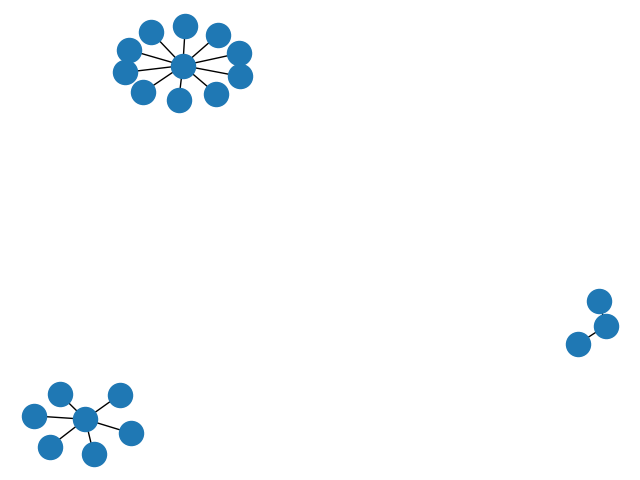
\includegraphics[scale=0.3]{Router}
	\caption{Router}
	\label{fig:Router}
\end{figure}
\section{Evaluation and Result}

\subsection{Baselines}
Given two nodes x and y be the node we want to predict. We let the set of neighbor x be N(x). We implemented six very common heuristics. And we organized the six heuristics in \ref{tab:method}. \\
\subsubsection{Common Neighbors(CN)}
It is a very simple heuristic. Two nodes have more common neighbor will be more likely to have a link. The score can represented as $|N(x) \cap N(y)|$.
\subsubsection{Jaccard(JC)}
It is very similar to common neighbors. If x and y are high degree nodes, it is not surprised that they will have many common neighbors. Jaccard wants to consider this effect and put the size of union of the neighbors of two nodes in denominator. It can be represented as $\frac{|N(x) \cap N(y)|}{|N(x) \cup N(y)|}$
\subsubsection{Adamic Adar(AA)}
It is also very similar to common neighbors. Given the assumption that a low degree common neighbor have more contribution to probability that x and y having a link. We divide the weight of each common neighbor by the logarithm of its degree. It is actually very similar to a TFIDF. And we can represented Adamic Adar as $\sum_{z \in N(x) \cap N(y)}{\frac{1}{log(|N(z)|)}}$
\subsubsection{Total Neighbors(TN)}
It is the most simple baseline which is just to calculate the total size of neighbors of x and y. It can be represented as $|N(x)| + |N(y)|$
\subsubsection{Preferential Attachment(PA)}
Given the assumption that a high degree nodes have more chance to have link have other nodes. Preferential Attachment calculate the product of degree of x and y. It can be represented as $|N(x)| * |N(y)|$
\subsubsection{Page Rank(PG)}
It is very similar to PA. But instead of just using the degree product of nodes, it use the product of the score after performing page rank to our network. Because the product can be very small, we use the sum of logarithm instead. Let $r_x$ be the score of x after performing page rank and $r_y$ be the score of y after performing page rank. It can be represented as $\log{r_x} + \log{r_y}$
\begin{table}
	\begin{center}
		\begin{tabular}{|c|c|}
			\hline
			method & description \\
			\hline
			common neighbor(CN) & $|N(x) \cap N(y)|$ \\
			Jaccard(JC) & $\frac{|N(x) \cap N(y)|}{|N(x) \cup N(y)|}$ \\
			Adamic and Adar(AA) & $\sum_{z \in N(x) \cap N(y)}{\frac{1}{log(|N(z)|)}}$ \\
			Total Neighbor(TN) & $|N(x)| + |N(y)|$ \\
			Preferentail Attachment (PA) & $|N(x)| * |N(y)|$ \\
			Page Rank(PR)  & $\log{r_x} + \log{r_y}$ \\	
			\hline
		\end{tabular}
	\end{center}
\caption{link prediction methods}
\label{tab:method}
\end{table}

\subsection{Evaluation}
Evaluation is not a trivial problem when it comes to link prediction problem. If we want to do all pair evaluation, it will take O($N^2$) predictions where N is the size of the nodes. And even for a small graph with 1000 nodes, the evaluation time is not trivial.
 
In fact, make a fair and effective evaluation is also a research topic and Ryan and Nitech has published a paper of how to evaluate link prediction problem. We choose the most common way to evaluate our model which is to do down-sampling on negative samples. 

We randomly divide our edges into training, validation and testing according to the ratio 0.8:0.1:0.1. Training set is only for training, validation set is only for grid search of best parameters, and testing set is only for evaluate our model.

For validation and testing we randomly sample negative samples that equal to their size. If it is unlucky enough, some nodes may only exists in validation or testing set and not exist in training set, in this case, we will discard this edges in the evaluation.

To evaluate our result, we mainly use AUC score(area under Receiver Operating Characteristics). Because AUC has a very good characteristic which is the sampling AUC is actually an approximation of actual AUC even if we do down-sampling in negative data set. 

However, if our model rank all positive data that higher than 90 percent of negative data but all of the positive data not the top ranked. The AUC score will be great ($>0.9$) but all of the positive data are not likely to be recommended. Therefore, we also implement f1@k score as an evaluation. For the parameter k, we temporaily set the k equal to the size of positive label. For this k, recall is actually equal to precision. And it has a very intuitive physical meaning which is "the accuracy of finding all of the missing link if we know the size of missing link". In the future, we'll try to set different k and see the influence of the k. 

\section{Result and Discussion}
\begin{table}
	\begin{center}
		\begin{tabular}{|c|c|c|c|c|c|c|}
		\hline
		Data Set & CN & JAC & AA & PA  & TN & PG \\
		\hline
		Celegans&0.8314&0.7669&0.8443&0.7554&0.734&0.7998\\
		facebook&0.9882&0.9863&0.9893&0.8324&0.7345&0.8198\\
		NS&0.9742&0.9747&0.9741&0.6803&0.5204&0.7062\\
		PB&0.9152&0.8669&0.9176&0.908&0.8776&0.9175\\
		Power&0.5965&0.5964&0.5965&0.528&0.5198&0.7757\\
		Router&0.6109&0.6102&0.6111&0.9298&0.9198&0.9659\\
		USAir&0.9509&0.9164&0.9626&0.9021&0.868&0.9188\\
		Yeast&0.902&0.901&0.9029&0.8561&0.7926&0.8864\\
		\hline
		\end{tabular}
	\end{center}
	\caption{AUC of the six baselines}
	\label{tab:auc}
\end{table}

\begin{table}
	\begin{center}
		\begin{tabular}{|c|c|c|c|c|c|c|}
			\hline
			Data Set & CN & JAC & AA & PA & TN & PG \\
			\hline
			Celegans&0.7407&0.5926&0.713&0.5694&0.5787&0.6296\\
			facebook&0.9546&0.9312&0.9544&0.6742&0.5618&0.655\\
			NS&0.9524&0.9524&0.9524&0.5281&0.3939&0.4935\\
			PB&0.8052&0.6927&0.801&0.7762&0.7223&0.7846\\
			Power&0.1947&0.1947&0.1947&0.396&0.3518&0.5199\\
			Router&0.2279&0.2279&0.2279&0.761&0.7574&0.8272\\
			USAir&0.8278&0.7608&0.8612&0.799&0.7799&0.7608\\
			Yeast&0.815&0.815&0.815&0.7024&0.6184&0.7274\\
			\hline
		\end{tabular}
	\end{center}
	\caption{F1 score of the six baselines}
	\label{tab:f1}
\end{table}

Table \ref{tab:auc} shows AUC of six different baselines and table \ref{tab:f1} shows F1 score of the six baselines. 

According to the result, we can see that no heuristic method can outperform all other heuristics.  And we can see that Adamic Adar(AA), Jaccard, and common neighbors perform pretty well in facebook, NS data set. However, in power and router data set. The result of common neighbor based method are pretty bad. It is not surprised because that in power and router data set, there are few triangles and thus common neighbor might not be a good heuristic. 

\section{Future Work}
We want to keep working on what we have proposed in our proposal. Because we already finish our evaluation framework, we can start implement our machine learning models. And the result will be included in our final report. 



\bibliographystyle{acm}
\bibliography{midterm_progress_report}


\end{document}